\section{Sport-Recht-Sicherheit}

\begin{question}{3}
Was verstehen Sie unter der Eigenverantwortlichkeit des Schneesportlers?
\end{question}
\begin{solution}
Schneesport darf grunds"atzlich "uberall in freier Natur betrieben werden, aber stets auf eigene Gefahr. Ein gewisses Ma"s an Gefahr ist naturgegeben und muss auf schneesportliche Weise bew"altigt werden.\\
Bereitschaft, im Schadensfall, Schuld bei sich zu suchen. Vorsicht und Reaktionsbereitschaft sind geboten.\\\\
\citetitle{theorie} Seite 103
\end{solution}

\begin{question}{6}
Was verstehen Sie unter der Verkehrssicherungspflicht und unter typischen und atypischen Gefahren? Nennen Sie hierf"ur jeweils vier Beispiele.
\end{question}
\begin{solution}
\emph{Verkehrssicherungspflicht:} Alle Pflichten, die derjenige auf sich nimmt, der ein Gel"ande dem "offentlichen Verkehr zug"anglich macht. Somit haben Bergbahn- und Liftgesellschaften daf"ur Sorge zu tragen, dass den Schneesportlern nichts passiert.\\
\emph{Atypische Gefahr:} Gefahr, die nicht vorhersehbar bzw. durch regelgerechtes Verhalten ver- mieden oder abgewendet werden kann.
\begin{itemize}
\item Gro"sfl"achige Vereisungen
\item Absturzgefahr innerhalb einer Abstandszone von zwei Metern neben dem Pistenrand
\item Lawinen
\item Gruppe/Verein steckt einen Lauf
\end{itemize}
\emph{Typische Gefahr:} Vorhersehbar und durch vorausschauendes Fahren abwendbar.
\begin{itemize}
\item Eisplatten und apere Stellen
\item Pistenraupen (pl"otzliches Auftauchen)
\item Begrenzungen etc.
\end{itemize}
\citetitle{theorie} Seite 104
\end{solution}

\begin{question}{3}
Erl"autern Sie den Unterschied zwischen organisiertem und freiem Skiraum.
\end{question}
\begin{solution}
\emph{Organisierter Skiraum:} Pisten und gesicherter Randbereich von ca. 2 Metern neben dem Pistenrand und Skirouten\\
\emph{Freier Skiraum:} "ubriges Gel"ande (Sportler bewegt sich hier auf eigene Gefahr)\\\\
\citetitle{theorie} Seite 106
\end{solution}

\begin{question}{4}
Erl"autern Sie den Unterschied zwischen einer geschlossenen und einer gesperrten Strecke. Beschreiben Sie m"ogliche Konsequenzen und Folgen, wenn Sie eine gesperrte Strecke befahren.
\end{question}
\begin{solution}
\emph{Geschlossene Strecke:} Befahren auf eigene Gefahr; Kein Anspruch auf Verkehrssicherung; Wird durch Anzeigetafel an Berg-/Talstation bekannt gegeben\\
\emph{Gesperrte Strecke:} Verbot der Streckennutzung, da Gef"ahrdung anderer; Anzeige durch gelb-schwarzes Sperrschild; Sperrung durch Verwaltungsbeh"orde\\
\emph{Konsequenzen:} Bu"sgelder; Gef"ahrdung anderer (Haftpflichtversicherung kann Zahlung im Schadensfall verweigern), wer eine gesperrte Strecke trotzdem bef"ahrt, handelt grob fahrl"assig oder gar vors"atzlich; Lawinen (Rettungsma"snahmen werden gef"ahrdet); Abfahrtsstrecke (Rennl"aufer wird gef"ahrdet)\\\\
\citetitle{theorie} Seite 108-110
\end{solution}

\begin{question}{3}
Erl"autern Sie die r"aumlichen, sachlichen und pers"onlichen Anwendungsbereiche der FIS-Regeln.
\end{question}
\begin{solution}
\emph{R"aumlicher Geltungsbereich:} Gesicherter Pisten- und Loipenbereich, freies Skigel"ande (Freeride- und Skitourbereich)\\
\emph{Sachlicher Geltungsbereich:} F"ur Alpinski sowie f"ur s"amtliche Sportger"ate, die durch ihre Gleiteigenschaften eine dem Skifahren vergleichbare Abfahrt erm"oglichen (= schwerkraftabh"angige Schnee- gleitger"ate)!entscheidend: technische M"oglichkeit, kantengesteuert zu fahren, die Richtung zu "andern und zu bremsen\\
\emph{Pers"onlicher Geltungsbereich:} F"ur jedermann, der am Schneesport teilnimmt.\\\\
\citetitle{theorie} Seite 111-112
\end{solution}

\begin{question}{2}
Nennen und erl"autern Sie die FIS-Verhaltensregeln 1/ 2/ 3/ 4/ 5/ 6/ 7/ 8/ 9/ 10 f"ur Ski- fahrer und Snowboarder.
\end{question}
\begin{solution}
\begin{enumerate}
\item \emph{R"ucksicht auf die anderen Skifahrer und Snowboarder:} Jeder Skifahrer/Snowboarder muss sich so verhalten, dass er keinen anderen gef"ahrdet oder sch"adigt.
\item \emph{Beherrschung der Geschwindigkeit und der Fahrweise:} Jeder Skifahrer/Snowboarder muss auf Sicht fahren. Er muss seine Geschwindigkeit und seine Fahrweise seinem K"onnen und den Gel"ande-, Schnee- und Witterungsverh"altnissen sowie der Verkehrsdichte anpassen.
\item \emph{Wahl der Fahrspur:} Der von hinten kommende Skifahrer/Snowboarder muss seine Fahrspur so w"ahlen, dass er vor ihm fahrende Skifahrer/Snowboarder nicht gef"ahrdet.
\item \emph{"uberholen:} "uberholt werden darf von oben oder unten, von rechts oder links, aber immer nur mit einem Abstand, der dem "uberholten Skifahrer/Snowboarder f"ur alle seine Bewegungen gen"ugend Raum l"asst.
\item \emph{Einfahren, Anfahren und hangaufw"arts Fahren:} Jeder Skifahrer/Snowboarder, der in eine Skiabfahrt einfahren, nach einem Halt wieder anfahren oder hangaufw"arts schwingen oder fahren will, muss sich nach oben und unten vergewissern, dass er dies ohne Gefahr f"ur sich und andere tun kann.
\item \emph{Anhalten:} Jeder Skifahrer/Snowboarder muss es vermeiden, sich ohne Not an engen oder un"ubersichtlichen Stellen einer Abfahrt aufzuhalten. Ein gest"urzter Skifahrer/Snowboarder muss eine solche Stelle so schnell wie m"oglich freimachen.
\item \emph{Aufstieg und Abstieg:} Ein Skifahrer/Snowboarder, der aufsteigt oder zu Fu"s absteigt, muss den Rand der Abfahrt benutzen.
\item \emph{Beachten der Zeichen:} Jeder Skifahrer/Snowboarder muss die Markierung und die Signalisation beachten.
\item \emph{Hilfeleistung:} Bei Unf"allen ist jeder Skifahrer/Snowboarder zur Hilfeleistung verpflichtet.
\item \emph{Ausweispflicht:} Jeder Skifahrer/Snowboarder, ob Zeuge oder Beteiligter, ob verantwortlich oder nicht, muss im Falle eines Unfalls seine Personalien angeben.
\end{enumerate}
\citetitle{theorie} Seite 488-489
\end{solution}

\begin{question}{2}
Beschreiben Sie kurz die Voraussetzungen zur Gr"undung eines rechtsf"ahigen Vereins.
\end{question}
\begin{solution}
\begin{itemize}
\item Mindestmitgliederzahl 7 Personen, \S 56 BGB
\item Satzung (Vereinszweck, Sitz des Vereins, Ziel, dass der Verein eingetragen werden soll), \S 57 BGB
\item Rechtsf"ahigkeit wird mit Eintragung erlangt
\item Eintragung nach \S\S 59-66 BGB
\end{itemize}
\citetitle{theorie} Seite 116
\end{solution}

\begin{question}{7}
Beschreiben Sie die Aufsichtspflicht. Nennen sie dabei die Art und Kriterien sowie die Anforderungen an die Erf"ullung der Aufsichtspflicht.
\end{question}
\begin{solution}
\emph{Rechtsgrundlage der Aufsichtspflicht:} Gesetzlich: z.B. Aufsichtspflicht von Eltern f"ur ihre Kinder, \S\S 1626 ff. BGB; Vertraglich durch die vereinbarte "ubernahme, z.B. Kinderbetreuer, DSV-"ubungsleiter\\
\emph{Art der Aufsichtspflicht:} Aufsicht "uber Minderj"ahrige zum Schutz Dritter vor Sch"adigung durch den Aufsichtsbed"urftigen; Aufsicht zur Verhinderung von Sch"aden am Aufsichtsbed"urftigen (Obhutspflicht); Sorgfaltspflicht\\
\emph{Kriterien der Aufsichtspflicht:} Alter; Geistige F"ahigkeiten; Charakter; Vorhersehbarkeit des Schadenseintritts; Objektive Anforderungen der konkreten Situation\\
\emph{Anforderungen an die Erf"ullung der Aufsichtspflicht:}\\
Allgemein: Vorsorgliche Belehrung und Warnung; St"andige "Uberwachung; Eingreifen soweit erforderlich\\
Speziell an die Lehrkraft: Gef"ahrdungsfreies Vermitteln der Skitechnik; Vermeiden unn"otiger Gefahren f"ur sich und andere; "Uberpr"ufung der Ausr"ustung; Niemanden zum Mitfahren zwingen (Fahren "uber die Verh"altnisse vermeiden); FIS-Regeln und DSV-Tipps schulen und deren Einhaltung "uberwachen\\\\
\citetitle{theorie} Seite 119-120
\end{solution}

\begin{question}{4}
Nennen Sie die wichtigsten Inhalte einer Zielvereinbarung bei mehrt"agigen Schnee- sportkursen f"ur Kinder und Jugendliche mit "Ubernachtung.
\end{question}
\begin{solution}
\begin{itemize}
\item Inhalt und Rahmenprogramm der Ma"snahme
\item Hausordnung (Nachtruhe etc.)
\item Freizeitregelung (Ausgang, Gastst"attenbesuch etc.)
\item Keine Suchtstoffe (Alkohol, Nikotin, Drogen etc.)
\item Ausnahmen (ggf. bei Alkohol in geringen Mengen)
\item Festlegung von Folgen bei Verst"o"sen
\item Ausr"ustungshinweise
\item Versicherungshinweise (v.a. auch f"ur Ma"snahmen im Ausland)
\item Kostenregelung einschlie"slich Taschengeldempfehlung
\item Name, Anschrift und tel. Erreichbarkeit des Leiters, der Ausbilder und Betreuer oder, noch besser, gegenseitiger Austausch der Telefonnummern
\end{itemize}
\citetitle{theorie} Seite 127
\end{solution}

\begin{question}{4}
Sie sind mit einer Gruppe Kinder unter 14 Jahren/ Jugendliche zwischen 14 und 16 Jahren/ Jugendliche zwischen 16 und 18 Jahren auf einer Schneesportfreizeit. Erl"autern Sie relevante Bestimmungen des Jugendschutzgesetzes f"ur diese Altersgruppe.
\end{question}
\begin{solution}
Siehe Abbildung \ref{fig:js}
\begin{figure}[H]
  \centering
  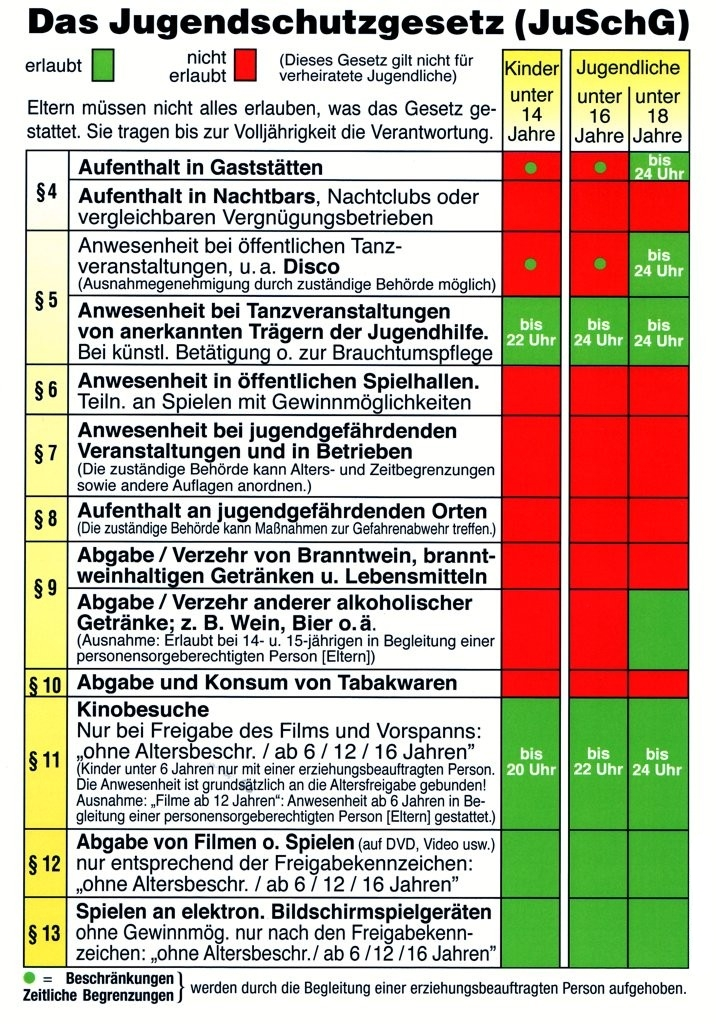
\includegraphics[width=8cm]{js.jpg}
  \caption{Jugendschutzgesetz Bestimmungen.}
  \label{fig:js}
\end{figure}
\citetitle{theorie} Seite 134
\end{solution}